\section{Results}
\label{sec:experiments_results}

This section reports the results of applying \gls{car} to the six environments described in Section~\ref{sec:experiments_configuration}.
Sections~\ref{ssec:initial_policy_training} and~\ref{ssec:surrogate_policy_training} first check that the two learning stages of the pipeline behave as expected: that the initial policies reach a competent level of play, and that the surrogate policies faithfully imitate them.
Section~\ref{ssec:experiments_latent_space_analysis} then presents the analysis of the latent representations and the values of the three evaluation metrics.

\subsection{Initial policy training}
\label{ssec:initial_policy_training}

\begin{figure}[t]
    \centering
    \resizebox{\textwidth}{!}{
    \begin{tikzpicture}
    \begin{axis}[
        xlabel={Training iteration},
        ylabel={Mean episode return (\% of best reached)},
        grid=major, ymajorgrids=true,
        xmin=0, ymin=0, ymax=105,
        width=\textwidth, height=0.5\textwidth,
        legend style={at={(0.5,-0.22)}, anchor=north, legend columns=3,
            /tikz/every even column/.append style={column sep=0.4cm}},
    ]
        \addplot[color=breakoutColor, mark=\breakoutMark, mark size=\breakoutMarkSize] coordinates {(1,0.1) (211,19.3) (421,19.3) (631,23.6) (841,30.6) (1051,40.7) (1261,52.1) (1471,23.4) (1681,38.3) (1891,58.2) (2101,45.0) (2311,34.8) (2521,55.6) (2731,54.7) (2941,39.5) (3151,68.5) (3361,60.2) (3571,68.8) (3781,42.2) (3991,52.1) (4201,35.7) (4411,45.7) (4621,45.0) (4831,43.5) (5041,53.8) (5050,74.5)};
        \addlegendentry{Breakout}
        \addplot[color=marioBrosColor, mark=\marioBrosMark, mark size=\marioBrosMarkSize] coordinates {(1,0.3) (188,1.3) (375,2.3) (562,6.3) (749,16.5) (936,42.2) (1123,56.5) (1310,68.2) (1497,69.0) (1684,68.8) (1871,73.5) (2058,68.5) (2245,66.9) (2432,61.5) (2619,72.4) (2806,73.5) (2993,70.6) (3180,71.7) (3367,72.3) (3554,72.5) (3741,75.1) (3928,74.9) (4115,80.4) (4302,85.0) (4489,80.4) (4507,84.9)};
        \addlegendentry{Mario Bros}
        \addplot[color=msPacmanColor, mark=\msPacmanMark, mark size=\msPacmanMarkSize] coordinates {(1,0.8) (268,43.8) (535,69.4) (802,87.5) (1069,93.4) (1336,89.3) (1603,95.1) (1870,89.7) (2137,87.2) (2404,88.6) (2671,95.0) (2938,87.7) (3205,92.7) (3472,75.6) (3739,72.9) (4006,74.7) (4273,79.5) (4540,72.3) (4807,73.8) (5074,81.3) (5341,79.6) (5608,69.1) (5875,71.5) (6142,72.7) (6409,70.5) (6425,59.4)};
        \addlegendentry{Ms.\ Pac-Man}
        \addplot[color=pongColor, mark=\pongMark, mark options={line width=1.5pt, scale=1}, mark size=\pongMarkSize] coordinates {(1,0.0) (22,8.9) (43,20.6) (64,47.1) (85,80.8) (106,84.4) (127,87.8) (148,90.1) (169,91.5) (190,92.1) (211,93.0) (232,93.3) (253,94.3) (274,95.3) (295,95.8) (316,96.9) (337,96.4) (358,97.2) (379,97.5) (400,95.6) (421,97.5) (442,98.6) (463,98.7) (484,98.6) (505,99.5) (507,99.3)};
        \addlegendentry{Pong}
        \addplot[color=spaceInvadersColor, mark=\spaceInvadersMark, mark size=\spaceInvadersMarkSize] coordinates {(1,5.3) (192,29.3) (383,42.8) (574,45.6) (765,58.2) (956,51.4) (1147,41.6) (1338,49.8) (1529,56.5) (1720,53.3) (1911,66.3) (2102,66.9) (2293,74.4) (2484,67.1) (2675,66.3) (2866,58.4) (3057,62.3) (3248,72.8) (3439,79.7) (3630,78.2) (3821,81.9) (4012,81.3) (4203,75.6) (4394,81.6) (4585,75.4) (4604,75.7)};
        \addlegendentry{Space Invaders}
        \addplot[color=surroundColor, mark=\surroundMark, mark size=\surroundMarkSize] coordinates {(1,0.0) (298,17.2) (595,24.1) (892,36.6) (1189,33.3) (1486,44.4) (1783,45.6) (2080,60.1) (2377,73.6) (2674,82.8) (2971,87.2) (3268,88.4) (3565,90.0) (3862,92.8) (4159,92.0) (4456,93.6) (4753,95.3) (5050,94.0) (5347,96.4) (5644,95.2) (5941,97.8) (6238,96.0) (6535,96.3) (6832,98.5) (7128,97.9)};
        \addlegendentry{Surround}
    \end{axis}
    \end{tikzpicture}
    }
    \caption{Training of the initial policies with \gls{ppo}, one curve per environment.}
    \label{fig:initial_policy_training}
\end{figure}


Figure~\ref{fig:initial_policy_training} shows how the initial policies improve during \gls{ppo} training.
For each environment, the mean episode return is normalized so that $0\%$ and $100\%$ correspond to the lowest and highest mean return observed during that run.
In every environment the return increases and then reaches a plateau, at which point training is stopped.
The number of iterations required to reach this plateau varies from a few hundred, for Pong, to several thousand, for Surround and Ms.\ Pac-Man.
For Ms.\ Pac-Man the return decreases after its peak; since the best checkpoint is retained rather than the last one, this does not affect the policy that is subsequently analyzed.

To confirm that the trained policies play competently, their scores are compared with the reference scores reported by \cite{machado2017revisitingarcadelearningenvironment}.
Each initial policy reaches a score of the same order as these references, so it constitutes a reasonable target for imitation.

\subsection{Surrogate policy training}
\label{ssec:surrogate_policy_training}

\begin{figure}[t]
    \centering
    \resizebox{\textwidth}{!}{
    \begin{tikzpicture}
    \begin{axis}[
        ymode=log,
        xlabel={Epoch}, ylabel={Action loss},
        grid=major, ymajorgrids=true,
        xmin=0,
        width=\textwidth, height=0.5\textwidth,
        legend style={at={(0.5,-0.22)}, anchor=north, legend columns=3,
            /tikz/every even column/.append style={column sep=0.4cm}},
    ]
        \addplot[color=breakoutColor, mark=\breakoutMark, mark size=\breakoutMarkSize] coordinates {(1,3.3005) (34,0.7979) (67,0.4972) (100,0.3760) (133,0.3091) (166,0.2642) (199,0.2330) (232,0.2103) (265,0.1923) (298,0.1786) (331,0.1673) (364,0.1578) (397,0.1491) (430,0.1432) (463,0.1361) (496,0.1310) (529,0.1269) (562,0.1226) (595,0.1192) (600,0.1182)};
        \addlegendentry{Breakout}
        \addplot[color=breakoutColor, forget plot] coordinates {(1,3.3093) (34,0.8592) (67,0.5367) (100,0.4015) (133,0.3262) (166,0.2781) (199,0.2438) (232,0.2191) (265,0.2001) (298,0.1841) (331,0.1720) (364,0.1622) (397,0.1531) (430,0.1459) (463,0.1408) (496,0.1356) (529,0.1292) (562,0.1244) (595,0.1218) (600,0.1202)};
        \addplot[color=breakoutColor, forget plot] coordinates {(1,3.3299) (34,0.9590) (67,0.5697) (100,0.4143) (133,0.3293) (166,0.2777) (199,0.2418) (232,0.2167) (265,0.1969) (298,0.1820) (331,0.1700) (364,0.1597) (397,0.1515) (430,0.1439) (463,0.1382) (496,0.1314) (529,0.1275) (562,0.1228) (595,0.1195) (600,0.1184)};

        \addplot[color=marioBrosColor, mark=\marioBrosMark, mark size=\marioBrosMarkSize] coordinates {(1,14.8064) (6,6.6000) (11,4.6932) (16,3.7979) (21,3.2255) (26,2.7950) (31,2.4568) (36,2.1831) (41,1.9586) (46,1.7765) (51,1.6390) (56,1.5198) (61,1.4210) (66,1.3336) (71,1.2585) (76,1.1925) (81,1.1415) (86,1.0899) (91,1.0473) (96,1.0067) (100,0.9770)};
        \addlegendentry{Mario Bros}
        \addplot[color=marioBrosColor, forget plot] coordinates {(1,13.9914) (6,5.7239) (11,4.2091) (16,3.4875) (21,2.9882) (26,2.5980) (31,2.3031) (36,2.0587) (41,1.8517) (46,1.6883) (51,1.5464) (56,1.4302) (61,1.3393) (66,1.2574) (71,1.1879) (76,1.1276) (81,1.0730) (86,1.0292) (91,0.9897) (96,0.9535) (100,0.9291)};
        \addplot[color=marioBrosColor, forget plot] coordinates {(1,14.4070) (6,5.8056) (11,4.3536) (16,3.5892) (21,3.0552) (26,2.6428) (31,2.3269) (36,2.0684) (41,1.8752) (46,1.6995) (51,1.5680) (56,1.4471) (61,1.3526) (66,1.2709) (71,1.1982) (76,1.1348) (81,1.0816) (86,1.0358) (91,0.9926) (96,0.9550) (100,0.9270)};

        \addplot[color=msPacmanColor, mark=\msPacmanMark, mark size=\msPacmanMarkSize] coordinates {(1,27.1299) (12,4.8831) (23,2.4171) (34,1.4646) (45,1.0649) (56,0.8613) (67,0.7298) (78,0.6299) (89,0.5539) (100,0.4961) (111,0.4505) (122,0.4202) (133,0.3914) (144,0.3688) (155,0.3509) (166,0.3339) (177,0.3196) (188,0.3066) (199,0.2941) (200,0.2929)};
        \addlegendentry{Ms.\ Pac-Man}
        \addplot[color=msPacmanColor, forget plot] coordinates {(1,27.4661) (12,4.8214) (23,2.1927) (34,1.5704) (45,1.7119) (56,0.8459) (67,0.6609) (78,0.5625) (89,0.4881) (100,0.4401) (111,0.6438) (122,0.3744) (133,0.3474) (144,0.3299) (155,0.3120) (166,0.2957) (177,0.2860) (188,0.2749) (199,0.3547) (200,0.2608)};
        \addplot[color=msPacmanColor, forget plot] coordinates {(1,27.8892) (12,4.5449) (23,2.2309) (34,1.4869) (45,1.1135) (56,0.8831) (67,0.7563) (78,0.6963) (89,0.5726) (100,0.5595) (111,0.4733) (122,0.4310) (133,0.4060) (144,0.3792) (155,0.3794) (166,0.3522) (177,0.3243) (188,0.3117) (199,0.2987) (200,0.2966)};

        \addplot[color=pongColor, mark=\pongMark, mark options={line width=1.5pt, scale=1}, mark size=\pongMarkSize] coordinates {(1,2.5732) (6,1.3059) (11,0.9484) (16,0.7769) (21,0.6780) (26,0.6095) (31,0.5613) (36,0.5240) (41,0.4939) (46,0.4681) (51,0.4462) (56,0.4273) (61,0.4109) (66,0.3959) (71,0.3829) (76,0.3711) (81,0.3602) (86,0.3497) (91,0.3405) (96,0.3327) (100,0.3266)};
        \addlegendentry{Pong}
        \addplot[color=pongColor, forget plot] coordinates {(1,2.5733) (6,1.3004) (11,0.9744) (16,0.8094) (21,0.7182) (26,0.6519) (31,0.6026) (36,0.5607) (41,0.5261) (46,0.4978) (51,0.4728) (56,0.4510) (61,0.4325) (66,0.4157) (71,0.4007) (76,0.3878) (81,0.3759) (86,0.3657) (91,0.3560) (96,0.3475) (100,0.3415)};
        \addplot[color=pongColor, forget plot] coordinates {(1,2.5732) (6,1.3249) (11,0.9486) (16,0.7818) (21,0.6848) (26,0.6179) (31,0.5676) (36,0.5267) (41,0.4934) (46,0.4651) (51,0.4414) (56,0.4203) (61,0.4020) (66,0.3867) (71,0.3722) (76,0.3598) (81,0.3487) (86,0.3386) (91,0.3294) (96,0.3211) (100,0.3149)};

        \addplot[color=spaceInvadersColor, mark=\spaceInvadersMark, mark size=\spaceInvadersMarkSize] coordinates {(1,2.1788) (12,1.1213) (23,0.9292) (34,0.8281) (45,0.7546) (56,0.6980) (67,0.6508) (78,0.6127) (89,0.5793) (100,0.5531) (111,0.5309) (122,0.5113) (133,0.4946) (144,0.4799) (155,0.4667) (166,0.4549) (177,0.4442) (188,0.4347) (199,0.4264) (200,0.4260)};
        \addlegendentry{Space Invaders}
        \addplot[color=spaceInvadersColor, forget plot] coordinates {(1,2.1801) (12,1.1053) (23,0.9291) (34,0.8288) (45,0.7589) (56,0.7045) (67,0.6616) (78,0.6256) (89,0.5966) (100,0.5717) (111,0.5507) (122,0.5315) (133,0.5150) (144,0.5005) (155,0.4877) (166,0.4762) (177,0.4654) (188,0.4557) (199,0.4471) (200,0.4466)};
        \addplot[color=spaceInvadersColor, forget plot] coordinates {(1,2.1951) (12,1.1148) (23,0.9097) (34,0.8110) (45,0.7429) (56,0.6917) (67,0.6503) (78,0.6153) (89,0.5868) (100,0.5620) (111,0.5397) (122,0.5190) (133,0.5008) (144,0.4857) (155,0.4726) (166,0.4596) (177,0.4486) (188,0.4391) (199,0.4302) (200,0.4298)};

        \addplot[color=surroundColor, mark=\surroundMark, mark size=\surroundMarkSize] coordinates {(1,24.2212) (34,4.7912) (67,2.0912) (100,1.4291) (133,1.1316) (166,0.9598) (199,0.8497) (232,0.7670) (265,0.7080) (298,0.6612) (331,0.6230) (364,0.5919) (397,0.5663) (430,0.5424) (463,0.5225) (496,0.5059) (529,0.4896) (562,0.4765) (595,0.4648) (600,0.4626)};
        \addlegendentry{Surround}
        \addplot[color=surroundColor, forget plot] coordinates {(1,24.0464) (34,2.8642) (67,1.8330) (100,1.3987) (133,1.1628) (166,1.0158) (199,0.9126) (232,0.8353) (265,0.7736) (298,0.7260) (331,0.6858) (364,0.6513) (397,0.6234) (430,0.5987) (463,0.5766) (496,0.5572) (529,0.5407) (562,0.5243) (595,0.5112) (600,0.5088)};
        \addplot[color=surroundColor, forget plot] coordinates {(1,24.7783) (34,4.1007) (67,1.8595) (100,1.3125) (133,1.0589) (166,0.9075) (199,0.8081) (232,0.7370) (265,0.6835) (298,0.6427) (331,0.6093) (364,0.5809) (397,0.5578) (430,0.5374) (463,0.5206) (496,0.5050) (529,0.4904) (562,0.4782) (595,0.4662) (600,0.4658)};
    \end{axis}
    \end{tikzpicture}
    }
    \caption{Training action loss of the surrogate policies.}
    \label{fig:surrogate_policy_training}
\end{figure}


Figure~\ref{fig:surrogate_policy_training} shows, for each environment, the training action loss of the three surrogate policies: the mean squared error between the action-distribution parameters of the surrogate and those of the initial policy.
In every case the loss decreases smoothly, and the three independently trained policies follow almost identical trajectories, converging to the same value; the three curves in each panel largely overlap.
This consistency matters for \gls{car}: the method compares the latent representations of independently trained policies, and this comparison is only meaningful if these policies implement the same decision function.
The behavioral fidelity of the surrogate policies is quantified by the \BehaviorReconstructionName in the next section.

\subsection{Latent space analysis}
\label{ssec:experiments_latent_space_analysis}

We first evaluate the ability of the surrogate policies to replicate the behavior of the initial policies (\BehaviorReconstructionName, Table~\ref{tab:environments_metrics}).
Across all environments, the surrogate policies achieve an average \BehaviorReconstructionName of $0.95 \pm 0.02$, indicating that they reliably reproduce the decisions of the initial policies over 100 evaluation episodes.

\begin{table}[t]
\centering
\resizebox{\linewidth}{!}{
    \begin{tblr}{
        colspec={|c|c|c|c|},
        hlines,
        vlines,
        row{1} = {font=\bfseries, halign=c, valign=m}
    }
        Environment     & {\textit{Behavior} \\ \textit{Reconstruction}} & {\textit{Abstraction} \\ \textit{Score}} & {\textit{Clustering} \\ \textit{Universality}} \\
        Breakout        & 0.83 $\pm$0.03 & 0.82 $\pm$0.07 & 0.48 $\pm$0.11 \\
        Mario Bros      & 0.99 $\pm$0.03 & 0.71 $\pm$0.14 & 0.55 $\pm$0.10 \\
        Ms.\ Pac-Man    & 1.00 $\pm$0.03 & 0.43 $\pm$0.09 & 0.65 $\pm$0.08 \\
        Pong            & 0.95 $\pm$0.01 & 0.99 $\pm$0.00 & 0.49 $\pm$0.05 \\
        Space Invaders  & 0.97 $\pm$0.07 & 0.69 $\pm$0.06 & 0.67 $\pm$0.07 \\
        Surround        & 1.00 $\pm$0.01 & 0.55 $\pm$0.07 & 0.61 $\pm$0.09 \\
    \end{tblr}
}
\caption{Evaluation of \BehaviorReconstructionName, \AbstractionScoreName and \ClusteringUniversalityName across the six Atari environments.}
\label{tab:environments_metrics}
\end{table}

\FloatBarrier

For the remainder of the analysis, a random subset of 50,000 observations is embedded into the \gls{ls} of each surrogate policy, using the representation extracted directly after the last convolutional layer, and the resulting point cloud $\textcolor{myblue}{\mathcal{E}}$ is partitioned with $k$-means clustering \cite{macqueen1967multivariate}.

Across all environments, policies, and numbers of clusters, the average \AbstractionScoreName is $0.99 \pm 0.00$.
This indicates that the clusters formed in the \gls{ls} are not mere reflections of the raw pixel inputs or of the action distributions.

\begin{figure}[t]
    \centering
    \resizebox{\textwidth}{!}{
    \begin{tikzpicture}
    \begin{axis}[
        xlabel={Number of clusters},
        ylabel={\ClusteringUniversalityName},
        grid=major,
        xmin=1, xmax=30,
        ymin=0, ymax=1,
        ytick distance=0.25,
        ymajorgrids=true,
        width=\textwidth,
        height=0.55\textwidth,
        set layers=standard,
        legend style={at={(0.5,-0.22)}, anchor=north, legend columns=3,
            /tikz/every even column/.append style={column sep=0.4cm}},
    ]
        \addplot[color=breakoutColor, mark=\breakoutMark, mark size=\breakoutMarkSize] coordinates {
            (2,0.99) (3,0.39) (4,0.37) (5,0.70) (6,0.43) (7,0.50) (8,0.44) (9,0.41) (10,0.45) (11,0.51) (12,0.41) (13,0.41) (14,0.49) (15,0.54) (16,0.46) (17,0.48) (18,0.46) (19,0.46) (20,0.50) (21,0.50) (22,0.46) (23,0.49) (24,0.47) (25,0.47) (26,0.46) (27,0.44) (28,0.44) (29,0.39) (30,0.46)
        };
        \addlegendentry{Breakout}
        \addplot[color=marioBrosColor, mark=\marioBrosMark, mark size=\marioBrosMarkSize] coordinates {
            (2,0.98) (3,0.80) (4,0.50) (5,0.62) (6,0.62) (7,0.59) (8,0.51) (9,0.57) (10,0.52) (11,0.53) (12,0.45) (13,0.51) (14,0.47) (15,0.49) (16,0.51) (17,0.51) (18,0.50) (19,0.49) (20,0.55) (21,0.53) (22,0.53) (23,0.53) (24,0.52) (25,0.52) (26,0.52) (27,0.54) (28,0.51) (29,0.51) (30,0.52)
        };
        \addlegendentry{Mario Bros}
        \addplot[color=msPacmanColor, mark=\msPacmanMark, mark size=\msPacmanMarkSize] coordinates {
            (2,0.91) (3,0.75) (4,0.62) (5,0.59) (6,0.67) (7,0.78) (8,0.77) (9,0.71) (10,0.79) (11,0.69) (12,0.66) (13,0.69) (14,0.62) (15,0.60) (16,0.59) (17,0.61) (18,0.60) (19,0.60) (20,0.64) (21,0.63) (22,0.60) (23,0.67) (24,0.56) (25,0.54) (26,0.60) (27,0.62) (28,0.55) (29,0.58) (30,0.64)
        };
        \addlegendentry{Ms.\ Pac-Man}
        \addplot[color=pongColor, mark=\pongMark, mark options={line width=1.5pt, scale=1}, mark size=\pongMarkSize] coordinates {
            (2,0.59) (3,0.59) (4,0.49) (5,0.46) (6,0.51) (7,0.57) (8,0.60) (9,0.54) (10,0.48) (11,0.50) (12,0.47) (13,0.48) (14,0.44) (15,0.47) (16,0.44) (17,0.46) (18,0.44) (19,0.47) (20,0.45) (21,0.45) (22,0.51) (23,0.49) (24,0.46) (25,0.49) (26,0.50) (27,0.49) (28,0.52) (29,0.42) (30,0.47)
        };
        \addlegendentry{Pong}
        \addplot[color=spaceInvadersColor, mark=\spaceInvadersMark, mark size=\spaceInvadersMarkSize] coordinates {
            (2,0.81) (3,0.72) (4,0.93) (5,0.69) (6,0.74) (7,0.76) (8,0.61) (9,0.62) (10,0.67) (11,0.59) (12,0.59) (13,0.56) (14,0.61) (15,0.63) (16,0.69) (17,0.64) (18,0.65) (19,0.67) (20,0.67) (21,0.66) (22,0.65) (23,0.64) (24,0.69) (25,0.67) (26,0.67) (27,0.70) (28,0.68) (29,0.68) (30,0.66)
        };
        \addlegendentry{Space Invaders}
        \addplot[color=surroundColor, mark=\surroundMark, mark size=\surroundMarkSize] coordinates {
            (2,0.85) (3,0.74) (4,0.80) (5,0.72) (6,0.67) (7,0.67) (8,0.67) (9,0.69) (10,0.66) (11,0.72) (12,0.59) (13,0.67) (14,0.64) (15,0.60) (16,0.54) (17,0.52) (18,0.55) (19,0.55) (20,0.53) (21,0.54) (22,0.55) (23,0.55) (24,0.54) (25,0.59) (26,0.54) (27,0.52) (28,0.53) (29,0.54) (30,0.55)
        };
        \addlegendentry{Surround}
        \addplot[domain=1:30, color=white, very thick, on layer=axis foreground]{0.5};
        \addplot[domain=1:30, samples=2, color=black, very thick, dashed, on layer=axis foreground]{0.5};
    \end{axis}
    \end{tikzpicture}
    }
    \caption{Evolution of \ClusteringUniversalityName with respect to the number of clusters.}
    \label{fig:clustering_universality_curves}
\end{figure}


\begin{figure}[t]
    \centering
    \resizebox{\textwidth}{!}{
    \begin{tikzpicture}

    % ==============================
    % Part A (2 clusters)
    % ==============================
    \node at (0, 2cm) {\textbf{(A) The case with 2 clusters.}};

    \node (ligne_1) at (0, 0) {};

    \node[] at ($(ligne_1) + (-3.5cm, 0cm)$) {
    \begin{minipage}{8.5cm}
        \centering
        \begin{tikzpicture}
            % First image
            \node[anchor=south west,inner sep=0] (image1) at (0,0) {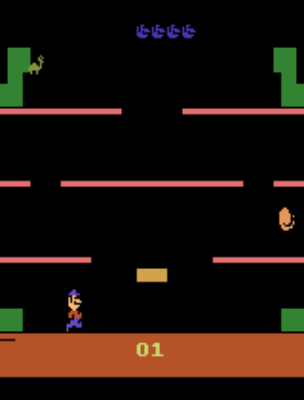
\includegraphics[width=2cm]{figures/clustering_agent_representation/pictures/mario_bros/2_clusters/bloc_pow_available/image_1.png}};
            \begin{scope}[shift={(image1.south west)}, x={(image1.south east)}, y={(image1.north west)}]
                \draw[red, line width=1pt] (0.4,0.275) rectangle (0.6,0.355);
            \end{scope}

            % Second image
            \node[anchor=south west,inner sep=0] (image2) at (image1.south east) [xshift=0.05cm] {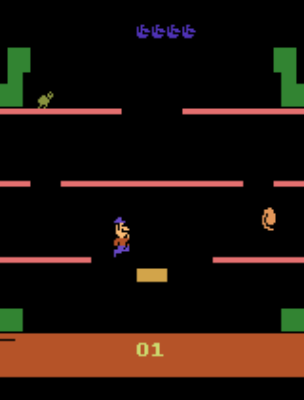
\includegraphics[width=2cm]{figures/clustering_agent_representation/pictures/mario_bros/2_clusters/bloc_pow_available/image_2.png}};
            \begin{scope}[shift={(image2.south west)}, x={(image2.south east)}, y={(image2.north west)}]
                \draw[red, line width=1pt] (0.4,0.275) rectangle (0.6,0.355);
            \end{scope}

            % Third image
            \node[anchor=south west,inner sep=0] (image3) at (image2.south east) [xshift=0.05cm] {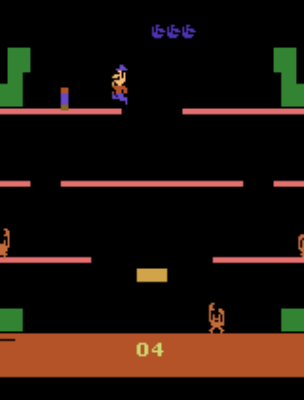
\includegraphics[width=2cm]{figures/clustering_agent_representation/pictures/mario_bros/2_clusters/bloc_pow_available/image_3.png}};
            \begin{scope}[shift={(image3.south west)}, x={(image3.south east)}, y={(image3.north west)}]
                \draw[red, line width=1pt] (0.4,0.275) rectangle (0.6,0.355);
            \end{scope}
        \end{tikzpicture}

        \small The POW block is present.
    \end{minipage}
    };

    \node[] at ($(ligne_1) + (3.5cm, 0cm)$) {
    \begin{minipage}{8.5cm}
        \centering
        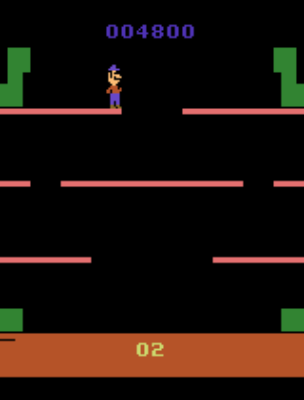
\includegraphics[width=2cm]{figures/clustering_agent_representation/pictures/mario_bros/2_clusters/bloc_pow_available_not/image_1.png}
        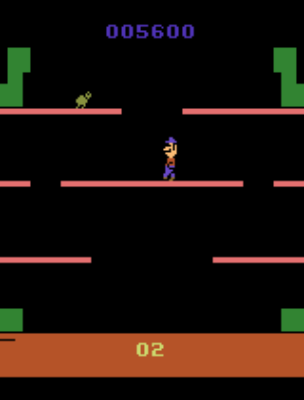
\includegraphics[width=2cm]{figures/clustering_agent_representation/pictures/mario_bros/2_clusters/bloc_pow_available_not/image_2.png}
        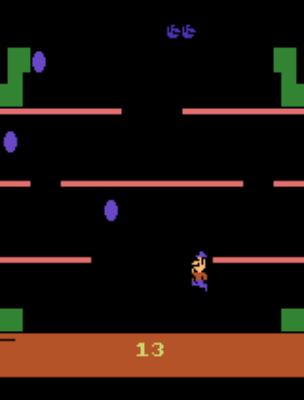
\includegraphics[width=2cm]{figures/clustering_agent_representation/pictures/mario_bros/2_clusters/bloc_pow_available_not/image_3.png}

        \small The POW block is absent.
    \end{minipage}
    };

    % ==============================
    % Separation line
    % ==============================
    \draw[dashed, thick] (-7,-2cm) -- (7,-2cm);

    % ==============================
    % Part B (5 clusters)
    % ==============================
    \node at (0, -2.5cm) {\textbf{(B) The case with 5 clusters.}};

    \node (ligne_2) at (0, -4.5cm) {};

    \node[] at ($(ligne_2) + (-4.5cm, 0cm)$) {
    \begin{minipage}{4.5cm}
        \centering
        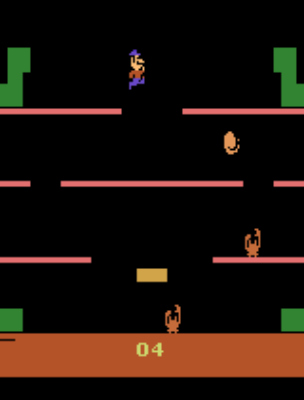
\includegraphics[width=2cm]{figures/clustering_agent_representation/pictures/mario_bros/5_clusters/bloc_pow_available/image_1.png}
        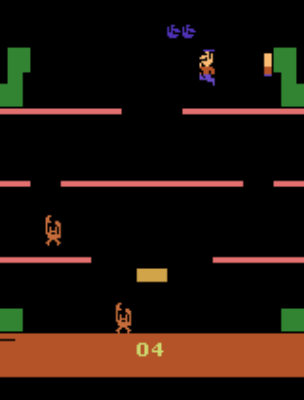
\includegraphics[width=2cm]{figures/clustering_agent_representation/pictures/mario_bros/5_clusters/bloc_pow_available/image_2.png}

        \small The POW block is present.
    \end{minipage}
    };

    \node[] at ($(ligne_2) + (0cm, 0cm)$) {
    \begin{minipage}{4.5cm}
        \centering
        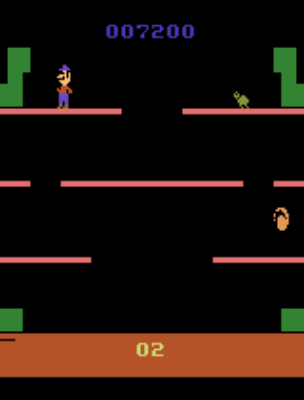
\includegraphics[width=2cm]{figures/clustering_agent_representation/pictures/mario_bros/5_clusters/move_on_top_left_platform/image_1.png}
        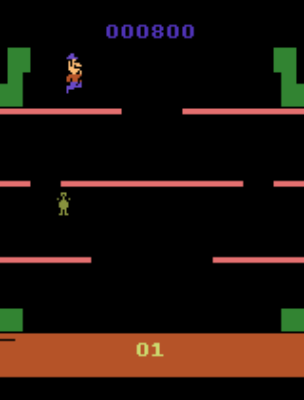
\includegraphics[width=2cm]{figures/clustering_agent_representation/pictures/mario_bros/5_clusters/move_on_top_left_platform/image_3.png}

        \small Move on the left platform.
    \end{minipage}
    };

    \node[] at ($(ligne_2) + (4.5cm, 0cm)$) {
    \begin{minipage}{4.5cm}
        \centering
        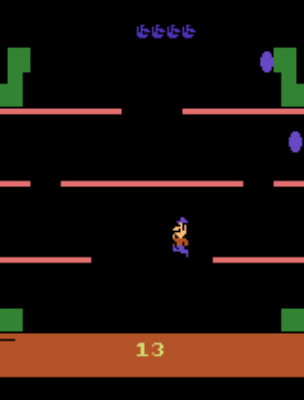
\includegraphics[width=2cm]{figures/clustering_agent_representation/pictures/mario_bros/5_clusters/move_through_level/image_1.png}
        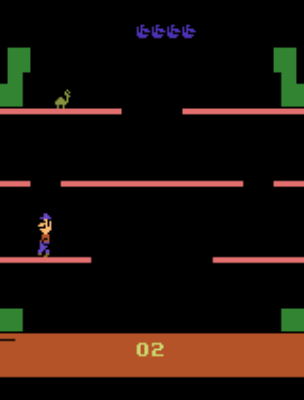
\includegraphics[width=2cm]{figures/clustering_agent_representation/pictures/mario_bros/5_clusters/move_through_level/image_2.png}

        \small Navigating through the level.
    \end{minipage}
    };

    \node[] (g5) at ($(ligne_2) + (-2.25cm, -3.5cm)$) {
    \begin{minipage}{4.5cm}
        \centering
        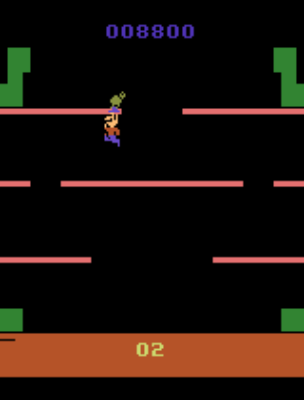
\includegraphics[width=2cm]{figures/clustering_agent_representation/pictures/mario_bros/5_clusters/neutralize_enemies_left/image_1.png}
        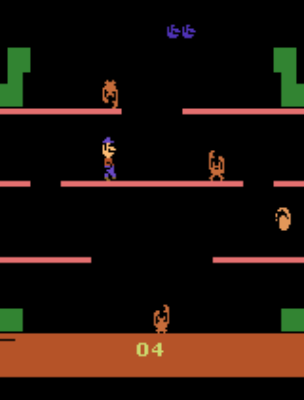
\includegraphics[width=2cm]{figures/clustering_agent_representation/pictures/mario_bros/5_clusters/neutralize_enemies_left/image_3.png}

        \small Attacking the left.
    \end{minipage}
    };

    \node[] at ($(ligne_2) + (2.25cm, -3.5cm)$) {
    \begin{minipage}{4.5cm}
        \centering
        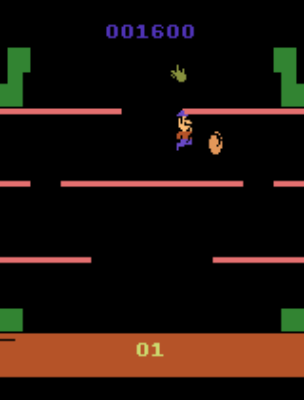
\includegraphics[width=2cm]{figures/clustering_agent_representation/pictures/mario_bros/5_clusters/neutralize_enemies_right/image_1.png}
        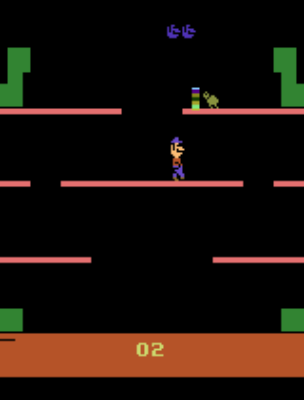
\includegraphics[width=2cm]{figures/clustering_agent_representation/pictures/mario_bros/5_clusters/neutralize_enemies_right/image_2.png}

        \small Attacking the right.
    \end{minipage}
    };

    \end{tikzpicture}
    }
    \caption{Effect of the number of clusters on the groupings identified by \gls{car} in the Mario Bros environment.}
    \label{fig:semantic_granularity}
\end{figure}


Figure~\ref{fig:clustering_universality_curves} reports the evolution of \ClusteringUniversalityName with respect to the number of clusters.
From three clusters onward, all curves stabilize around $0.5$ in every environment.
Since \ClusteringUniversalityName is computed from the \gls{ari}, this result indicates a strong similarity in the clustering of the \gls{ls} across surrogate policies within each environment \cite{amezquita2020orchestrating}, regardless of the number of clusters chosen.
This stability indicates that there is no single optimal number of clusters for explaining an agent's policy.
This raises the question of how many clusters should be selected to perform an analysis of \gls{ls}.
Our analysis suggests that this depends on the desired level of granularity.

With fewer clusters, \gls{car} highlights broad strategic patterns.
For instance, in the Mario Bros environment, the two main groups correspond to whether the POW block is present (highlighted in red in Figure~\ref{fig:semantic_granularity}A) or not.
This is particularly interesting, as the use of the POW block is a key determinant of strategy in this environment \cite{mario_bros_atari_2600}.

With a larger number of clusters, the analysis captures more fine-grained tactical behaviors, such as `Attacking the left.'' and `Navigating through the level.'' (see Figure~\ref{fig:semantic_granularity}B).

Both perspectives are valid, depending on whether the goal is to study strategic or tactical behaviors.
Similar interpretable structures can be observed across all evaluated environments.

% TODO: extend with the additional experimental material planned for this chapter:
% - ablation studies: analysed layer, clustering algorithm (K-means, GMM, deep embedding clustering),
%   distance measure, with/without action loss
% - deeper qualitative analysis of the discovered clusters
